\documentclass[10pt, a4paper]{article}

% --- Packages ---
\usepackage[utf8]{inputenc}
\usepackage[T1]{fontenc}
\usepackage{times} % Sets font to Times New Roman
\usepackage[margin=2.5cm]{geometry} % Sets 2.5cm margins
\usepackage{graphicx}
\usepackage{booktabs}          
\usepackage{microtype}
\usepackage{setspace}
\usepackage{titlesec}
\usepackage{sectsty}
\usepackage{cite}
\usepackage{float}
\usepackage{caption}
\usepackage{subcaption}
\usepackage{titling}
\usepackage{xurl}

% --- Settings ---
\singlespacing
\sectionfont{\normalsize}
\subsectionfont{\normalsize\it\bfseries}
\subsubsectionfont{\normalsize\it}
\setlength{\parindent}{0pt}
\captionsetup{font=normal}
\setlength{\droptitle}{-60pt}
\urlstyle{same}


% --- Preamble ---
\title{\Large \textbf{Intelligent UAV Systems for GNSS-Based Remote Sensing on Vegetation}}
\author{
    \normalsize\textbf{Student Team: }ZHOU Jiayi, MAHMUD Md Sahat, GAMAGE Sashenka, TAN Qing Lin \\
    \normalsize\textbf{Supervisors: }Prof. Guohao ZHANG, Prof. Li-Ta HSU
}
\date{\normalsize
    \it{Faculty of Engineering, the Hong Kong Polytechnic University}
}

\begin{document}
\maketitle

\section{Introduction}
The continuous and accurate monitoring of vegetation is essential for sustainable resource management and ecosystem preservation. Traditionally, vegetation monitoring relied on manual field assessments, which is highly dependent on the available expertise and resources \cite{Gibbons2006, Parkes2003}. To address these limitations and to accommodate for large-scale demands, remote sensing emerged as an essential tool.  

Remote sensing is the acquisition of information through measuring the energy reflected from the object of interest without direct contact \cite{campbell2011introduction}. Additionally, remote sensing could be classified into space-borne and airborne approaches. Space-borne remote sensing involves the use of instruments onboard satellites, including cameras \cite{Qian2022}, radars \cite{Hu2025}, and Light Detection and Ranging (LiDAR) sensors \cite{Bergen2009}. While space-borne methods can monitor macro-scale ecosystems over time, airborne remote sensing provides significantly improved resolution and flexibility through the integration of sensors onboard aircraft \cite{Khan2024}. Particularly, Unmanned Aerial Vehicles (UAVs) can be deployed on-demand with low costs, rendering them ideal for monitoring regional vegetation \cite{Tang2015}.

Among typical remote sensing payloads, LiDAR is particularly effective for vegetation monitoring due to its capacity to capture 3D information from spacially referenced point cloud environments. Additionally, unlike imaging instruments that are susceptible to lighting and weather, LiDAR measurements are more robust against varying illumination conditions and visually repetitive scenes, thus providing reliable geometric references of tree canopies \cite{Wu2024, jiang2025gps}. However, standalone LiDAR measurements lack global spatial context for a dynamic sensor platform \cite{wang2026multi}. Therefore, it is necessary to implement a Simultaneous Localization and Mapping (SLAM) framework to estimate the UAV trajectory while accurately constructing a spacial-referenced point cloud map.

Despite the demonstrated capabilities, LiDAR may face difficulties penetrating dense canopies \cite{Su2007}. Therefore, it is critical to explore additional sensing techniques that are low-power and low-weight to complement existing UAV payloads. Recently, the Global Navigation Satellite System Reflectometry (GNSS-R) is gaining increasing interest in the field of remote sensing. GNSS-R exploits the L-band signals transmitted from GNSS constellations that scatter on different Earth terrain surfaces, providing extensive information regarding the reflector on land \cite{Jin2024}. Additionally, any consumer-grade GNSS receiver can be used, demonstrating significant potential as low-cost UAV payloads.

While a GNSS-R system can obtain terrain information through the analytical characterization of reflected signals, the relationship between signal measurements and ground reflector features is often complex and non-linear. Therefore, in addition to the statistical analysis of GNSS-R data, machine learning models can also be leveraged for robust ground feature extraction. 

Lastly, the effectiveness of UAV-based remote sensing heavily depends on the efficiency of flight trajectories. While it is easy to assume the traditional lawnmower patterns common in robotics applications, they do not account for the unique ground reflection zone geometries inherent to an airborne GNSS-R system \cite{GALCERAN20131258, yu2021theory}. Consequently, an autonomous coverage path planning (CPP) framework is crucial for optimizing flight trajectories based on the corresponding GNSS satellite geometries \cite{Cabreira2019}. 

In summary, this project addresses the systemic gap for low-cost, intelligent, and multidisciplinary remote sensing systems through the following objectives: 

\begin{enumerate}
\item To introduce an autonomous path planning framework for optimized GNSS-R remote sensing.
\item To implement a SLAM framework for mapping vegetation in LiDAR-based environments.
\item To model the correlations between information retrieved through GNSS-R and ground conditions. 
\item To classify vegetation reflected signals and predict vegetation boundaries based on raw GNSS data.
\end{enumerate}

The code scripts of this project, a video demonstration of the final product, as well as sample datasets are organized into the GitHub repository \url{https://github.com/zhlouise/UAV_GNSS-R}.

\section{System Architecture}
\subsection{Logical Architecture}
Four core pipelines, each corresponding to a project objective, are integrated to form a systematic framework.

\begin{figure}[H]
    \centering
    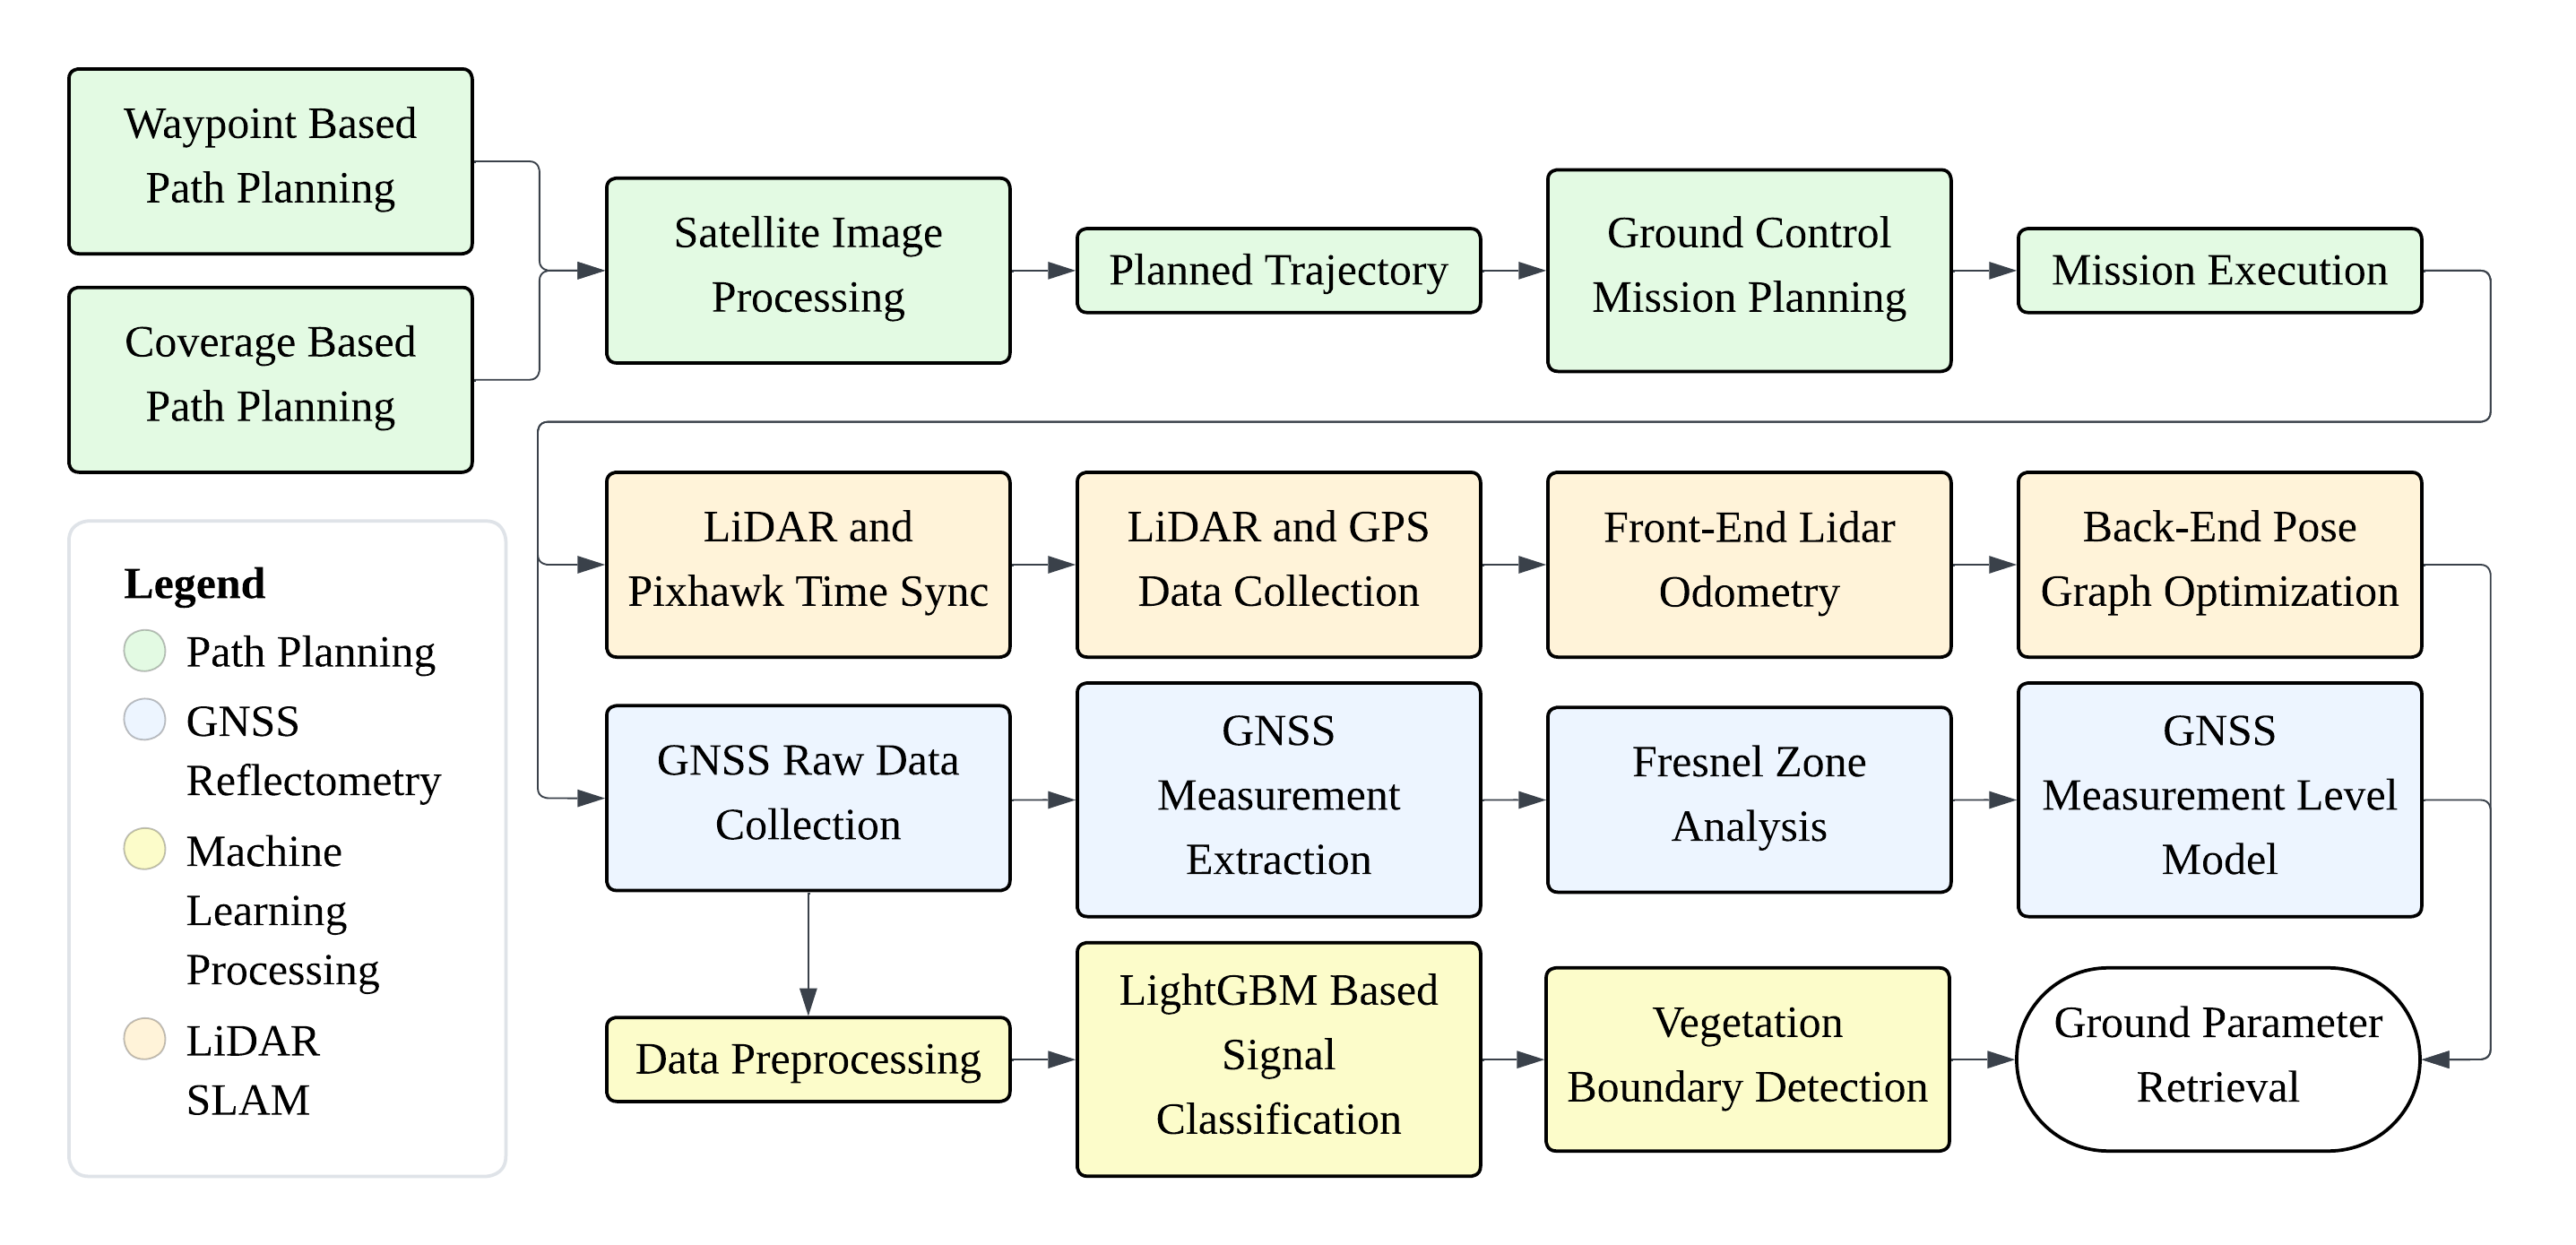
\includegraphics[width=0.85\textwidth]{Included_Images/System_Architecture.png}
    \caption{System Architecture}
\end{figure}

First, both waypoint-based and coverage-based path planning algorithms are adopted, while satellite imagery are used for identifying potential sensing regions. After designing the flight trajectory based on ground reflection zones of GNSS signals, the mission will be executed via ground control.

After the flight, the logged LiDAR data are time-synchronized. With both the LiDAR data and GPS solution time-stamped, both front-end LiDAR odometry and back-end Pose Graph Optimization (PGO) SLAM will be implemented for the generation of point cloud maps.

Simultaneously, the raw GNSS data collected during the flight mission are post-processed into two key measurements for analysis in correlation with the ground reflection zones - the First Fresnel Zones (FFZs). Such correlations will be modeled and used to retrieve ground parameters from GNSS-R measurements.

Lastly, a trained LightGBM machine learning model will be used to classify the received GNSS signals. The categorized vegetation-reflected signals will be used to detect vegetation boundary and cross-validate the ground parameters retrieved from the GNSS-R and LiDAR pipeline.

\subsection{Physical Architecture}
The UAV platform used is a Holybro X650 quadcopter with a Pixhawk 6C flight controller, linked to the ground control computer via telemetry radios. Onboard sensing instruments include a Livox Mid-360 LiDAR and a pair of U-blox F9P GNSS receivers, connected to an upward-facing antenna receiving direct signals and a downward-facing antenna receiving ground-reflected signals. The control and logging of sensor data are handled by an onboard Jetson Orin Nano Computer.

\begin{figure}[H]
    \centering
    \includegraphics[width=0.65\textwidth]{Included_Images/UAV_Setup.png}
    \caption{UAV Platform and Onboard Setup}
\end{figure}

\section{Methodology}

\subsection{Flight Trajectory Design}
To obtain optimal coverage of the target sensing area, the expected FFZs are calculated at target flight altitudes and time windows. Then, a nearest-neighbor distance clustering algorithm is employed to cluster the more concentrated FFZs as the primary region of interest. 

Since the resulting clusters are of irregular geometry, they are simplified into square, circular, or triangular shapes that maximize the spatial coverage of FFZs within the shape's enclosure. Then, the optimal trajectory separation is derived according to the cluster area, the desired overlap margin, and an empirical geometric shape factor specific to the cluster geometry.

\subsection{Point Cloud Map Generation}
The front-end LiDAR odometry utilizes the Fast-LIO framework, which operates via an Iterative Extended Kalman Filter (IEKF) that recursively updates the state vectors based on kinematic prediction models and measurement corrections. While forward kinematic predictions track system propagation and accumulate error covariances based on linearized Jacobian transition matrices, observed LiDAR feature scans modify the predictions through non-linear measurement models with sensor noises accounted. Lastly, an adaptive Kalman Gain is calculated across iterations to update the corrected covariance weights.

To mitigate inevitable long-term drifts, a back-end PGO pipeline is also adopted, where GPS positioning solutions regularly updates the trajectory while historical trajectory states are structured within a bipartite factor graph. The measurements are weighted by their respective inverse covariance matrices, while a Levenberg-Marquardt algorithm dynamically dampens the correction adjustments to account for multi-sensor residual errors. Lastly, extrinsic frame transformations handle rotational and translational offsets between the global GPS frame and the local LiDAR frame, providing corrected orientation at initialization.

\subsection{GNSS-R Signal Modeling}
The GNSS-R data collected during flight missions are post processed to extract each signal's carrier-to-noise ratio ($C/N_0$) and excess pseudorange delay. While $C/N_0$ represents the received carrier signal power relative to the noise power, the excess pseudorange delay represent the additional delay of the reflected signal after accounting for the geometric reflection delay. These parameters are then mapped to the corresponding FFZs to qualitatively analyze any correlations between GNSS signal characteristics and ground features. 

Additionally, the Pearson correlation coefficients between GNSS signal properties and the reference Color-Infrared (CIR) images are calculated to model the correlations between $C/N_0$, excess pseudorange delay, and ground feature infrared emission. This model is then used to reconstruct CIR information from GNSS signal parameters.

\subsection{Machine Learning Signal Classification}
As raw GNSS signal parameters are multidimensional and complex, a supervised LightGBM model is utilized to handle missing observations and classify the received signals without introducing manual input bias. In total, the model's feature vector includes five attributes obtained through the dual-antenna system: raw pseudorange, $C/N_0$, Doppler frequency shift, pseudorange error, and carrier phase. 

The database for training and testing consists of 70,125 distinct entries of three classes: 1) direct open-sky signals, 2) signals reflected over bare soil, and 3) signals reflected over vegetation. Then, the dataset is split according to the 60:20:20 ratio for training, testing, and validation. Lastly, a leaf-wise node growth approach is used to minimize the cross-entropy cost function and an extensive grid search configuration is used for hyperparameter fine-tuning for classification.

\section{Results and Discussion}

\subsection{Path Planning}
Among a total of 24 successful sensing flights conducted throughout the project, a field test was performed at Mount Davis Service Reservoir Garden, Hong Kong. Here, the autopilot was configured to maintain a continuous survey altitude of 35 meters, with a trajectory separation of 2 meters. 
\begin{figure}[H]
    \centering
    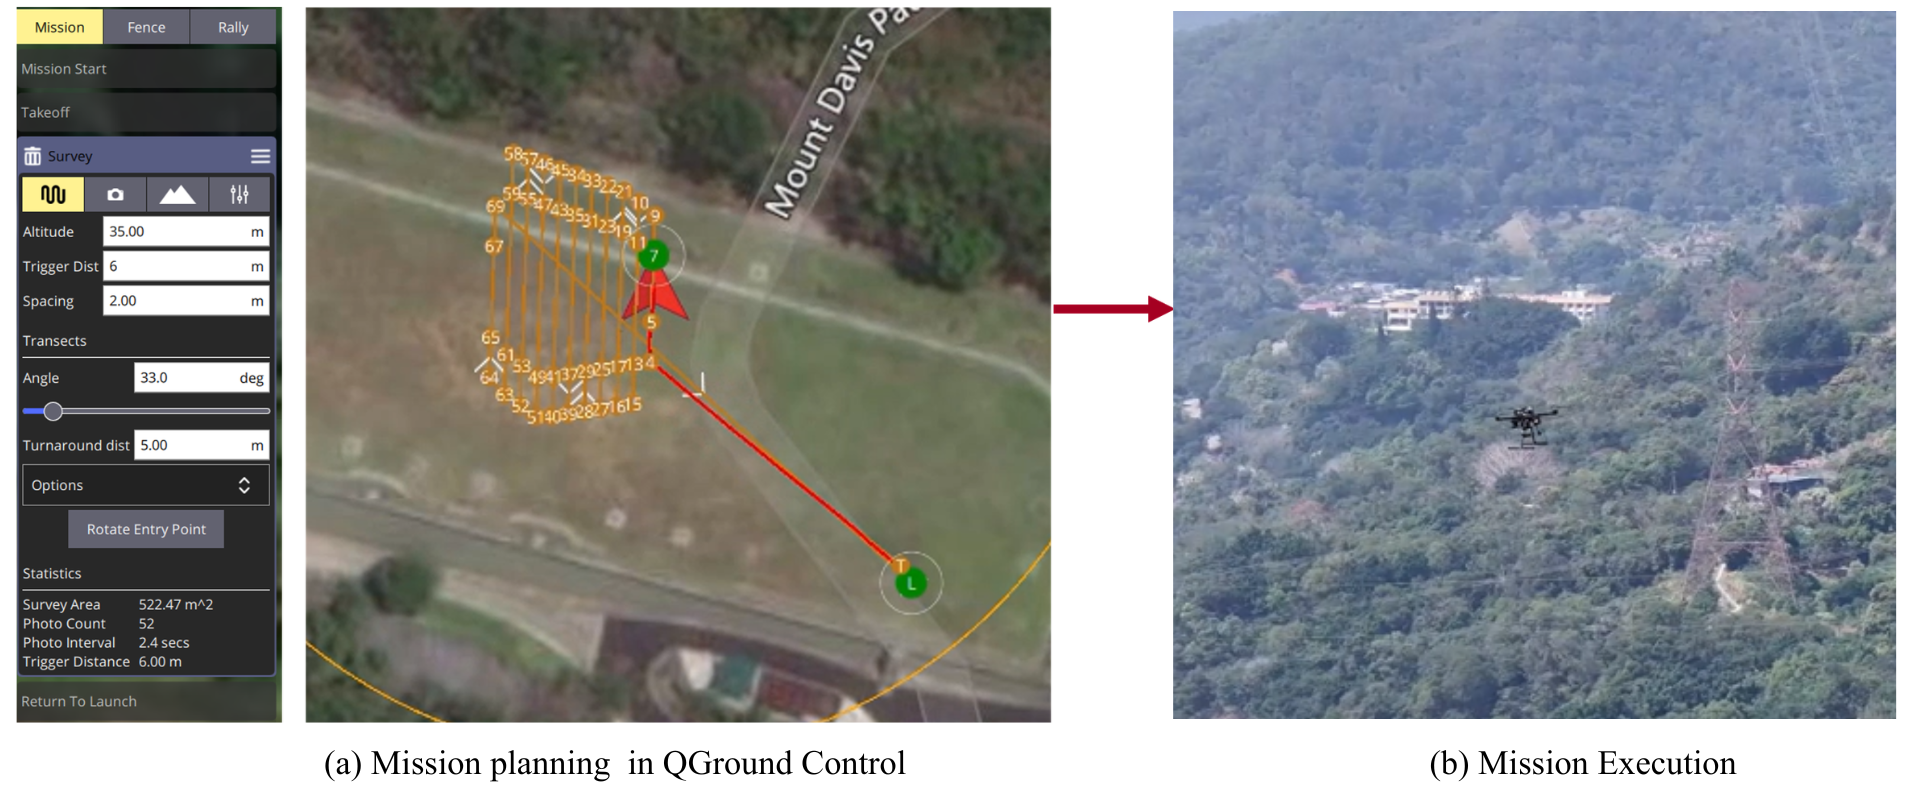
\includegraphics[width=0.75\textwidth]{Included_Images/KeyExperiment_Plannedpath.png}
    \caption{Mission Planning and Execution Results}
\end{figure}

\subsection{LiDAR SLAM}
To accurately map the ground conditions, the raw LiDAR logs were processed through both the standalone front-end odometry and the GPS-corrected back-end optimization. Here, both the front-end Fast-LIO odometry and the back-end PGO+GPS approaches present point clouds of different features, such as bare ground and tree canopies, which can be used as a geometric reference for GNSS-R derived vegetation areas.

\begin{figure}[H]
    \centering
    \begin{subfigure}{0.4\textwidth}
        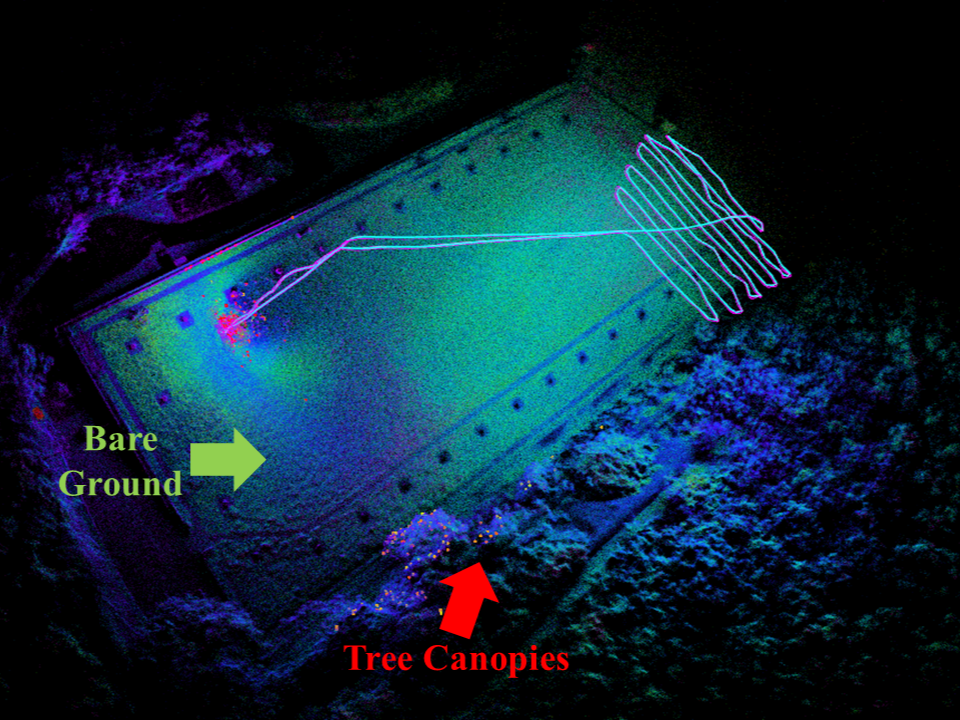
\includegraphics[width=\textwidth]{Included_Images/case_FL.png}
        \caption{Fast-LIO}
    \end{subfigure}
    \hfill
    \begin{subfigure}{0.4\textwidth}
        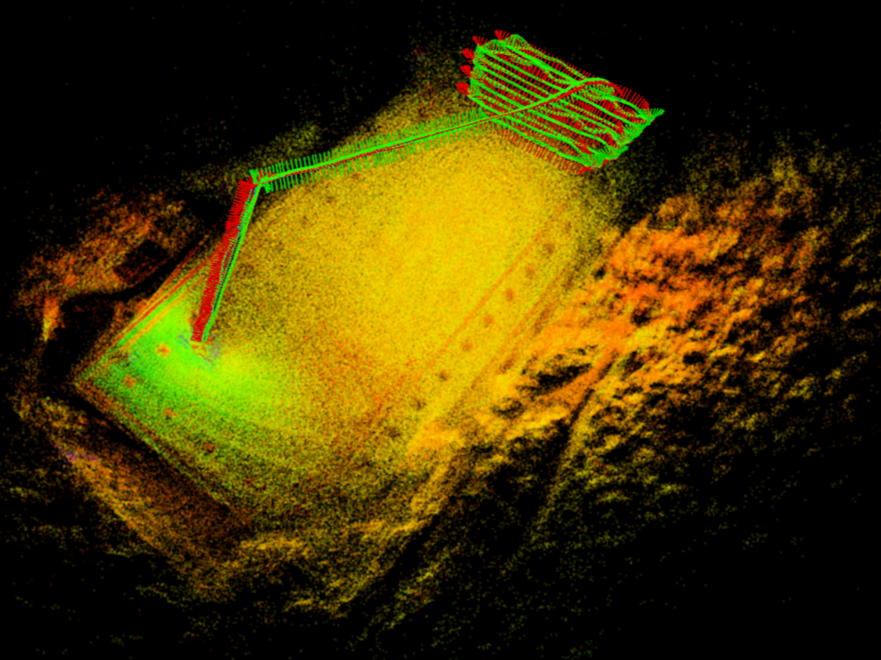
\includegraphics[width=\textwidth]{Included_Images/case_pgo.png}
        \caption{PGO+GPS}
    \end{subfigure}
    \caption{LiDAR SLAM results using two different techniques.}
\end{figure}

\subsection{GNSS-R}
The GNSS signal parameters captured distinguishing variations across unique ground boundaries. While the received $C/N_0$ ratios demonstrated significant differences between water bodies and vegetation canopies due to differences in dielectric properties, the excess pseudorange delays could distinguish sparse vegetation (grassy soil) from dense vegetation. Lastly, using the Pearson correlation coefficient models developed, the original CIR colors were constructed directly from the GNSS signal parameters for vegetation mapping.
\begin{figure}[H]
    \centering
    \begin{subfigure}{0.3\textwidth}
        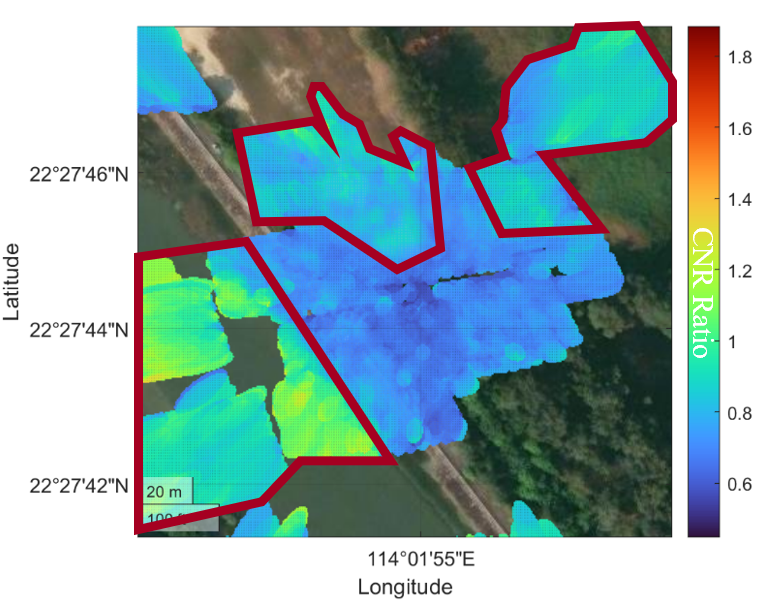
\includegraphics[width=\textwidth]{Included_Images/CNR_ratio_FFZ.png}
        \caption{$C/N_0$ Ratio}
    \end{subfigure}
    \hfill
    \begin{subfigure}{0.3\textwidth}
        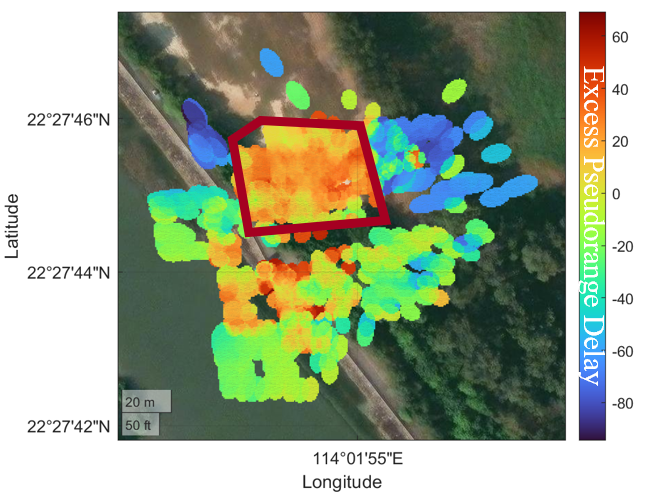
\includegraphics[width=\textwidth]{Included_Images/yuenlong_pr_delay.png}
        \caption{Excess Pseudorange Delay}
    \end{subfigure}
    \hfill
    \begin{subfigure}{0.3\textwidth}
        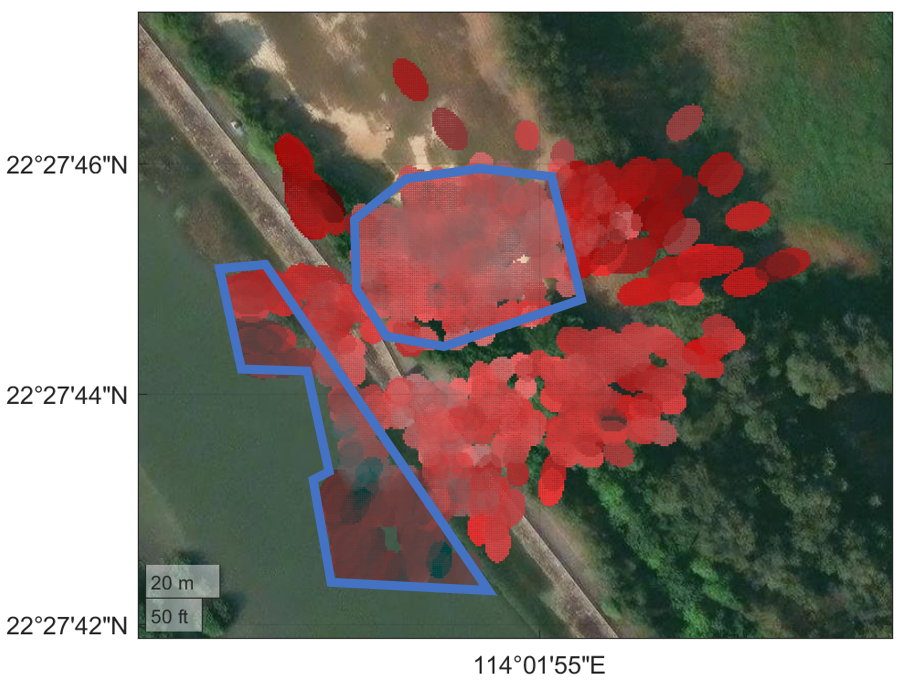
\includegraphics[width=\textwidth]{Included_Images/CIR_reconstruction_yuenlong.png}
        \caption{Reconstructed CIR Image Color}
    \end{subfigure}
    \caption{Received $C/N_0$ ratios, excess pseudorange delays, and reconstructed CIR color, plotted over the FFZs of the reflected signals.}
\end{figure}


\subsection{Machine Learning}
During training, the LightGBM classification model converged rapidly, narrowing the validation loss gap to a negligible margin. In testing evaluations, a predictive confidence score between 0.85 and 0.98 could be achieved for each satellite signal. Through projecting the classified signals into the centroids of their respective FFZ, the physical boundaries of the vegetation zones could be obtained. Moreover, the results aligned closely with the traditional analytical results from the GNSS-R data as well as the 3D features captured by LiDAR.

\begin{figure}[H]
    \centering
    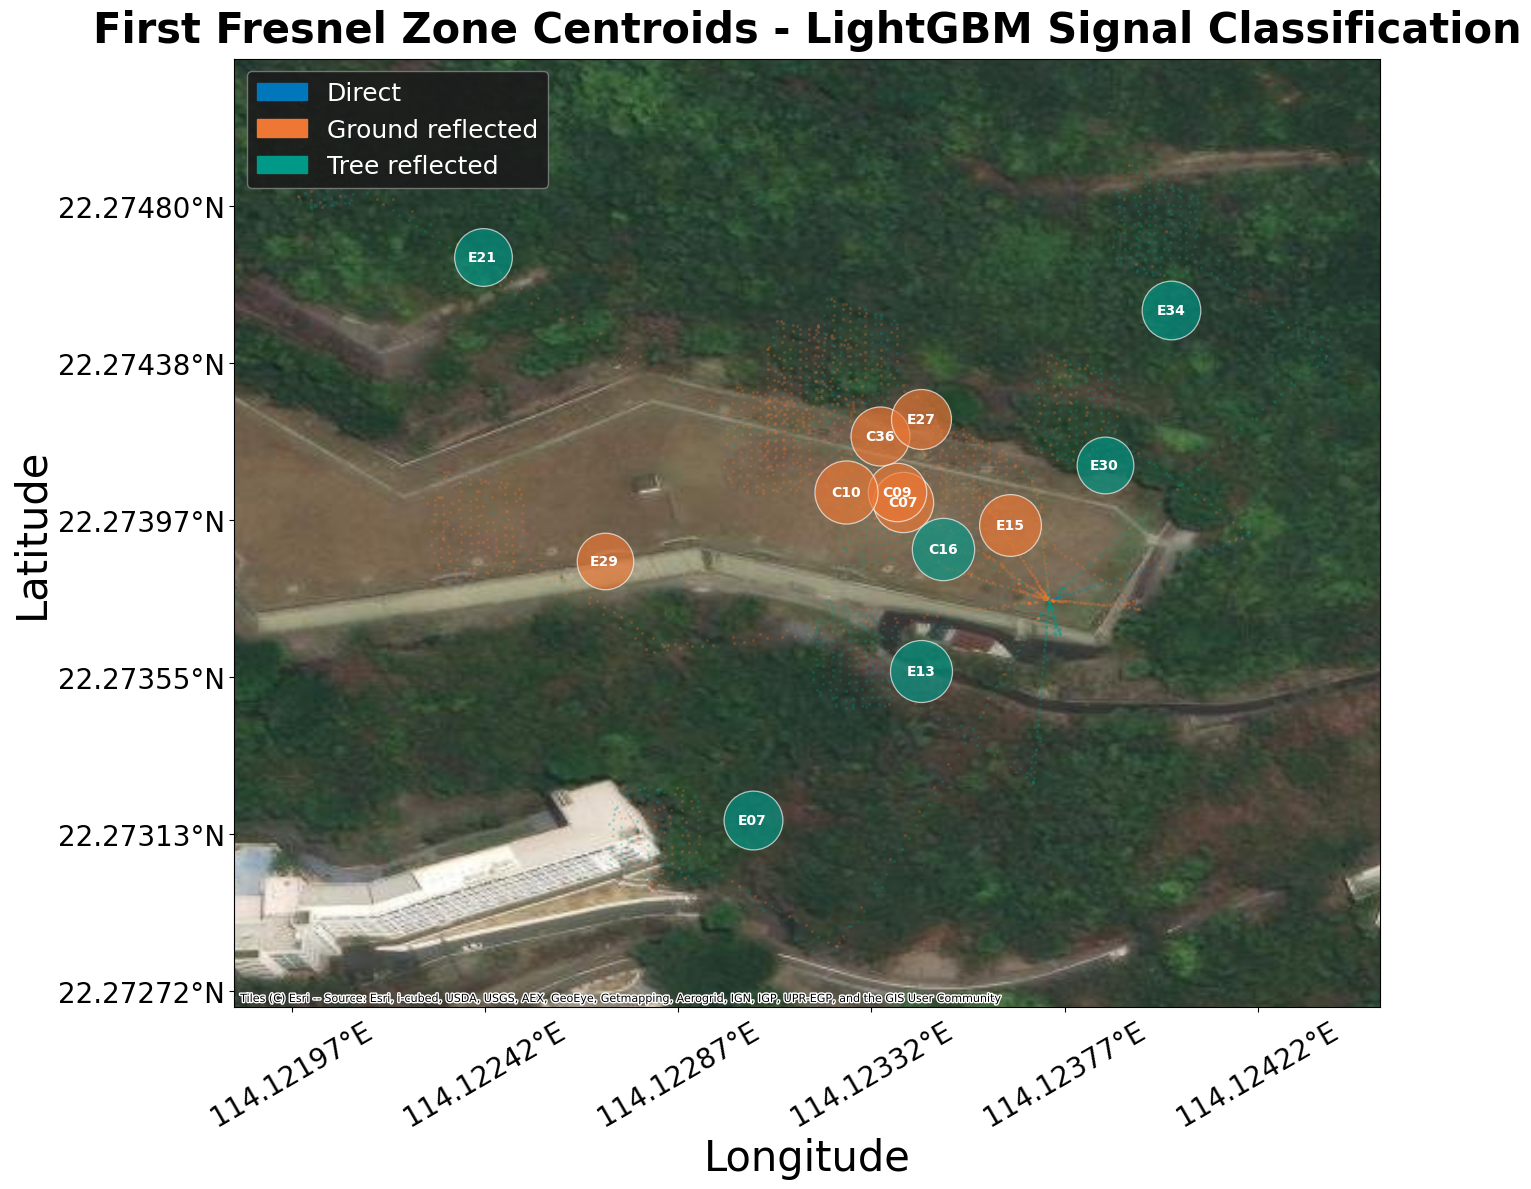
\includegraphics[width=0.55\textwidth]{Included_Images/mtdavis_ffzcon.png}
    \caption{Classified signals over FFZs, highlighting vegetation zones.}
\end{figure}

\section{Conclusion}
In conclusion, this project successfully established a comprehensive UAV-based framework for remote sensing, which integrates autonomous path planning for optimized vegetation coverage, LiDAR SLAM for accurate canopy mapping, GNSS-R for ground feature sensing, and machine learning for vegetation detection. 

While the integrated system achieved its primary objectives, it must be acknowledged that the project serves only as a demonstration for an intelligent UAV remote sensing system that possesses the potential for fully autonomous and streamlined local vegetation monitoring. The capability for the existing system majorly exists in offline post-processing of collected experimental data, while the use of GNSS signals for vegetation sensing applications remains a new topic. 

\section{Acknowledgements}
This project was completed under the guidance of chief supervisor Prof. Guohao ZHANG and co-supervisor Prof. Li-Ta HSU from the Department of Aeronautical and Aviation Engineering, The Hong Kong Polytechnic University. 

The student team acknowledges the use of open-source frameworks, toolkits, and data that supported this project:
\begin{itemize}
    \item The CPP algorithm was provided by the Boustrophedon Decomposition framework developed by the Autonomous Systems Lab at ETH Zurich.
    \item The Fast-LIO framework was adopted from the open-source repository developed by the Mechatronics and Robotic Systems Laboratory at the University of Hong Kong.
    \item The NASA Broadcast Ephemeris Data Products were used to determine the GNSS satellite coordinates.
    \item The raw GNSS data were processed using the RTKLIB and MatRTKLIB toolkits. 
    \item The above-ground altitude of the UAV was calculated using the Digital Terrain Model (DTM) provided by the Hong Kong Lands Department. 
    \item The reference CIR images were open sourced from the open-data portal of the Hong Kong Lands Department.
    \item The LightGBM model used for signal classification was based on the original framework developed by Microsoft.
\end{itemize}

\bibliographystyle{IEEEtran}
\bibliography{References.bib} 

\end{document}